\documentclass[dvipsnames,
%xcolor={svgnames},
hyperref={
	citecolor=blue,
	colorlinks=true,
	urlcolor=blue,
	linkcolor=,
}
]{beamer}
\beamertemplatenavigationsymbolsempty
\usetheme{Boadilla}
\usefonttheme[onlymath]{serif}

\usepackage{cleveref}

\usepackage{amsmath}
\usepackage{bm}
\usepackage{bbm}
\usepackage{mathrsfs}
\usepackage{mathtools}
\usepackage[cal=boondoxo]{mathalpha}

% Change horizontal spacing
\setlength{\tabcolsep}{3pt}

\usepackage[none]{hyphenat} % no hyphenation

\usepackage{array}

\usepackage{cancel}

\usepackage[style=authoryear,maxcitenames=2,backend=biber,citetracker=true]{biblatex}
\addbibresource{references.bib}

\usepackage{verbatim}

\usepackage{bigints}

\usepackage{makecell}

\usepackage{subcaption}

\DeclareCiteCommand{\citeauthor}
{\boolfalse{citetracker}%
	\boolfalse{pagetracker}%
	\usebibmacro{prenote}}
{\ifciteindex
	{\indexnames{labelname}}
	{}%
	\printtext[bibhyperref]{\printnames{labelname}}}
{\multicitedelim}
{\usebibmacro{postnote}}

\DeclareCiteCommand{\citeyear}
{\usebibmacro{prenote}}
{\bibhyperref{\printfield{year}}\bibhyperref{\printfield{extrayear}}}
{\multicitedelim}
{\usebibmacro{postnote}}

\newcommand{\credit}[2]{{\par\hfill \tiny #1 credit:~\itshape{\color{blue} \citeauthor{#2} (\citeyear{#2})}}}
\newcommand{\crediturl}[2]{{\par\hfill \tiny #1 credit:~\itshape{\color{blue} \url{#2}}}}
\let\oldcite\cite
\renewcommand{\cite}[1]{{\color{blue} \oldcite{#1}}}
\newcommand{\citefoot}[1]{{\color{blue} \citeauthor{#1} (\citeyear{#1})}}
\newcommand{\matr}[1]{#1}

\newcommand{\red}[1]{{\color{red} #1}}

\title[Deep Imbalanced Regression]
{\href{https://doi.org/10.48550/arXiv.2102.09554}{Deep Imbalanced Regression}}
%\subtitle{}
\author[Yang Y. et al.]{Yang Y, Zha K, Chen Y, Wang H, Katabi D}
%\institute{Aalto University}
\date{}%3 July 2024}

\addtobeamertemplate{title page}{}{
\begin{center}
\vspace{-5em}
ICML 2021
\\\vspace{4em}Presenter: Gianmarco Midena
\\\vspace{1em}26 November 2024
\end{center}}

\begin{document}
	
\begin{frame}
\titlepage
\end{frame}

\begin{frame}{Deep Imbalance Regression - Overview}
	\begin{figure}[h]
		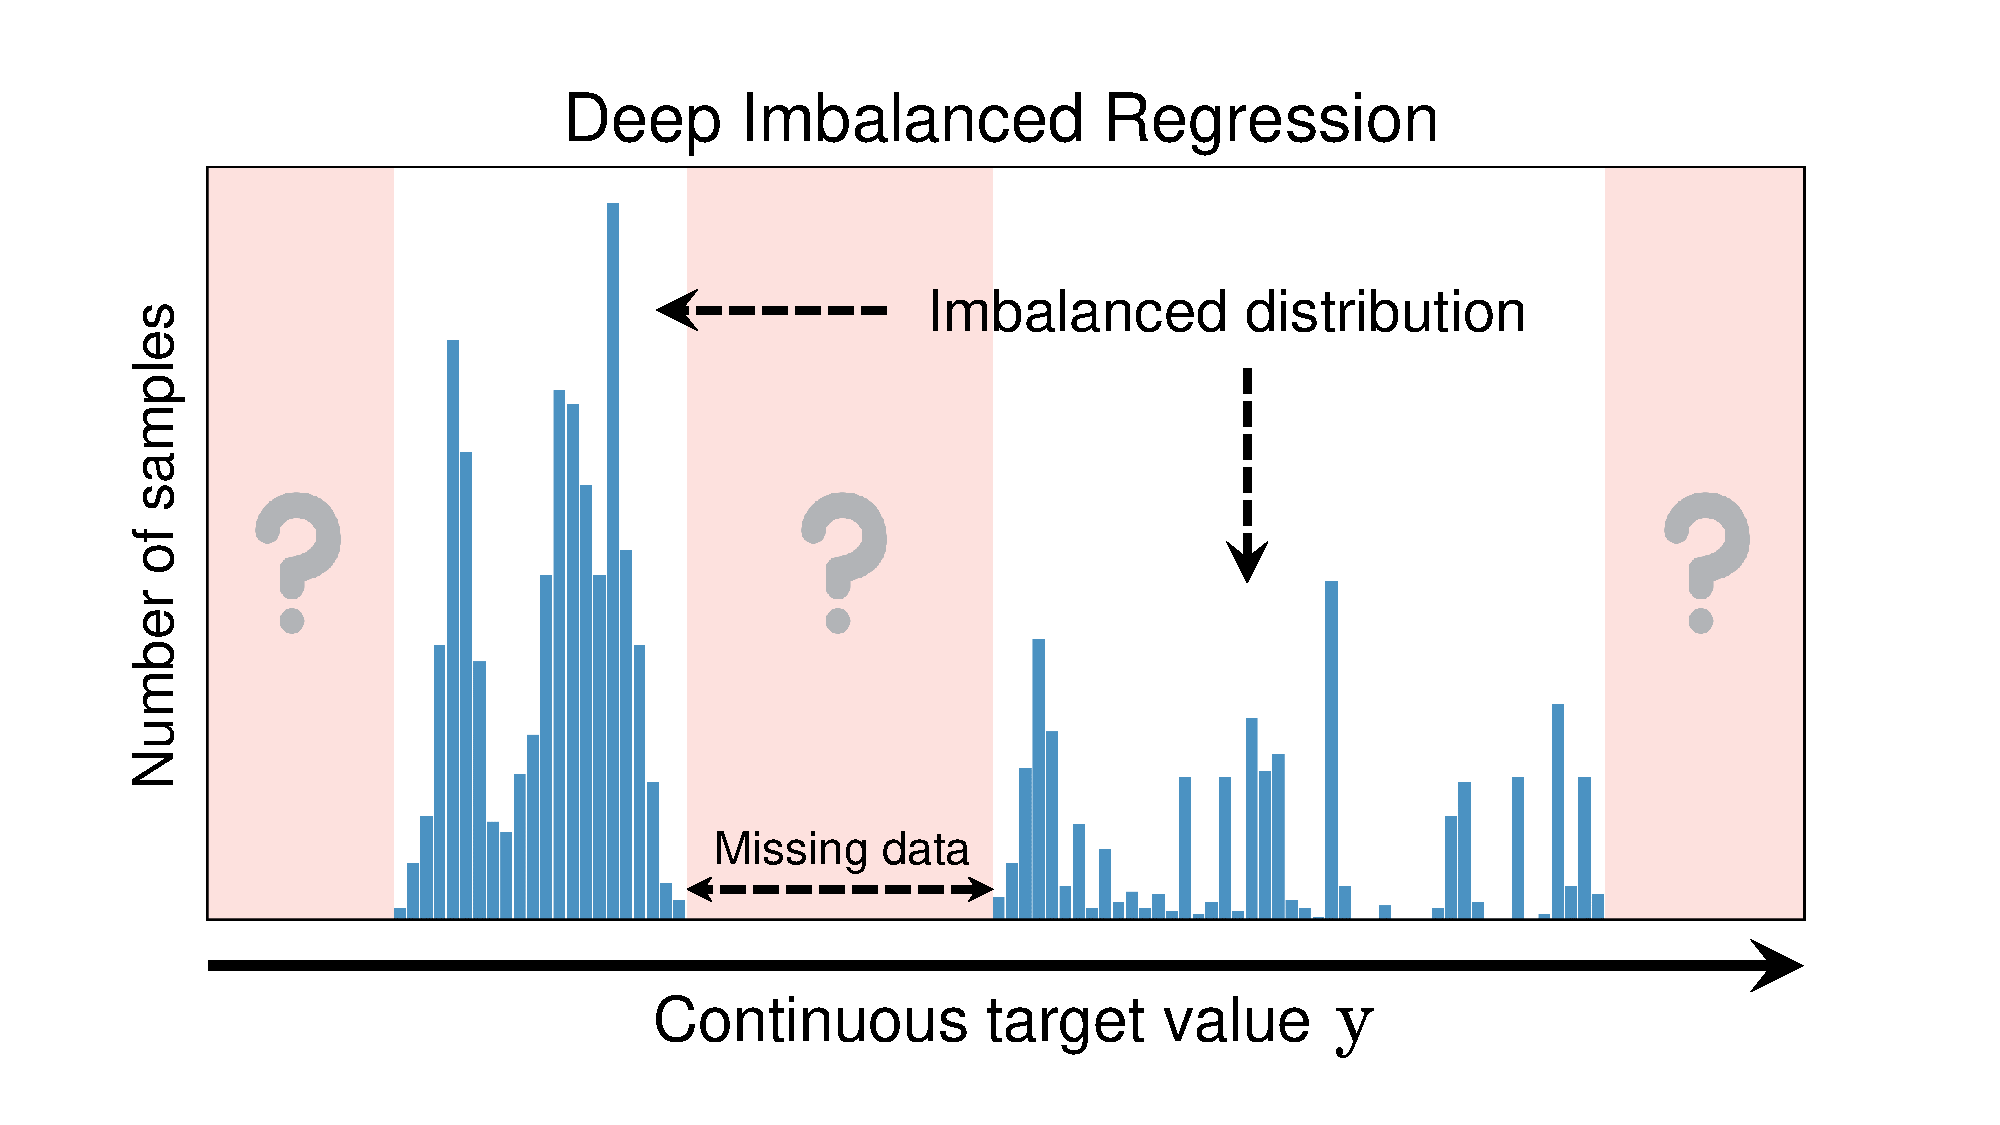
\includegraphics[width=\linewidth]{images/teaser.pdf}
		%\caption{}
	\end{figure}
	\credit{Image}{yang2021delving}
\end{frame}

\begin{frame}{Test Error on Categorical vs. Continuous Label Space}
	\begin{figure}[h]
	\begin{subfigure}{0.48\textwidth}
		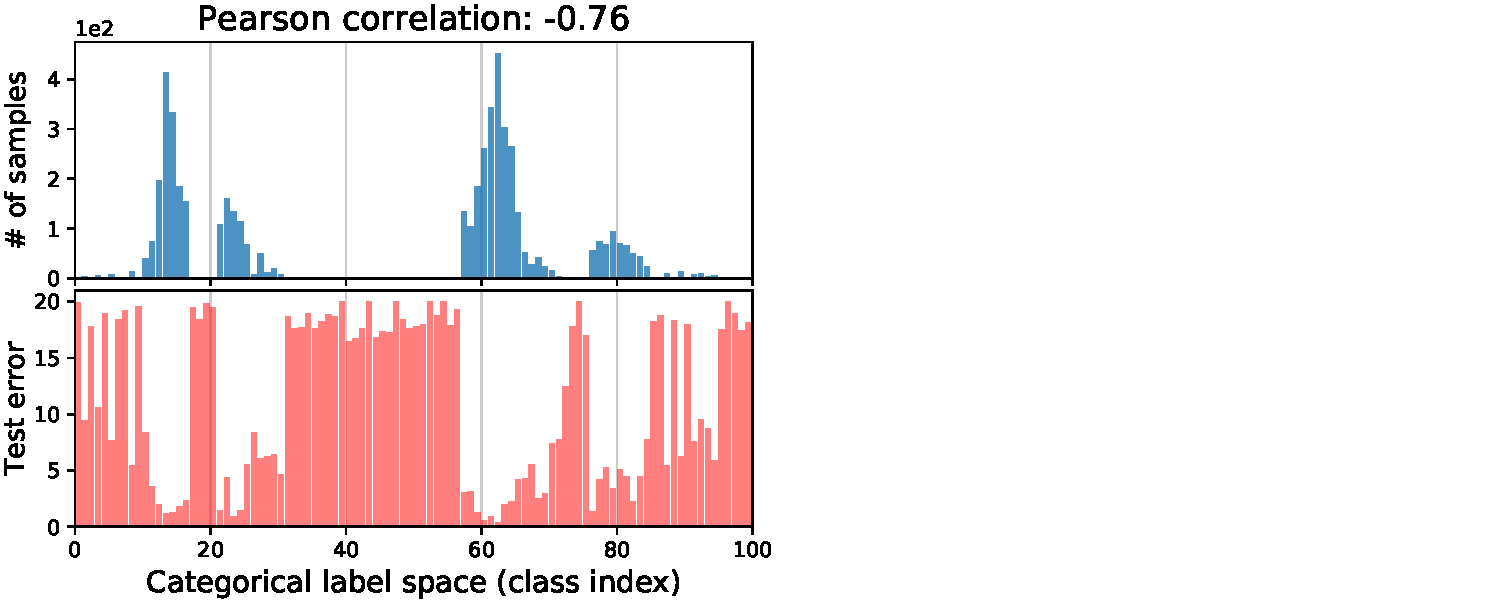
\includegraphics[width=\linewidth]{images/err_motivate_1_left.pdf}
		\caption{CIFAR-100 (subsampled)}
	\end{subfigure}\hspace{1em}%
	\begin{subfigure}{0.48\textwidth}
		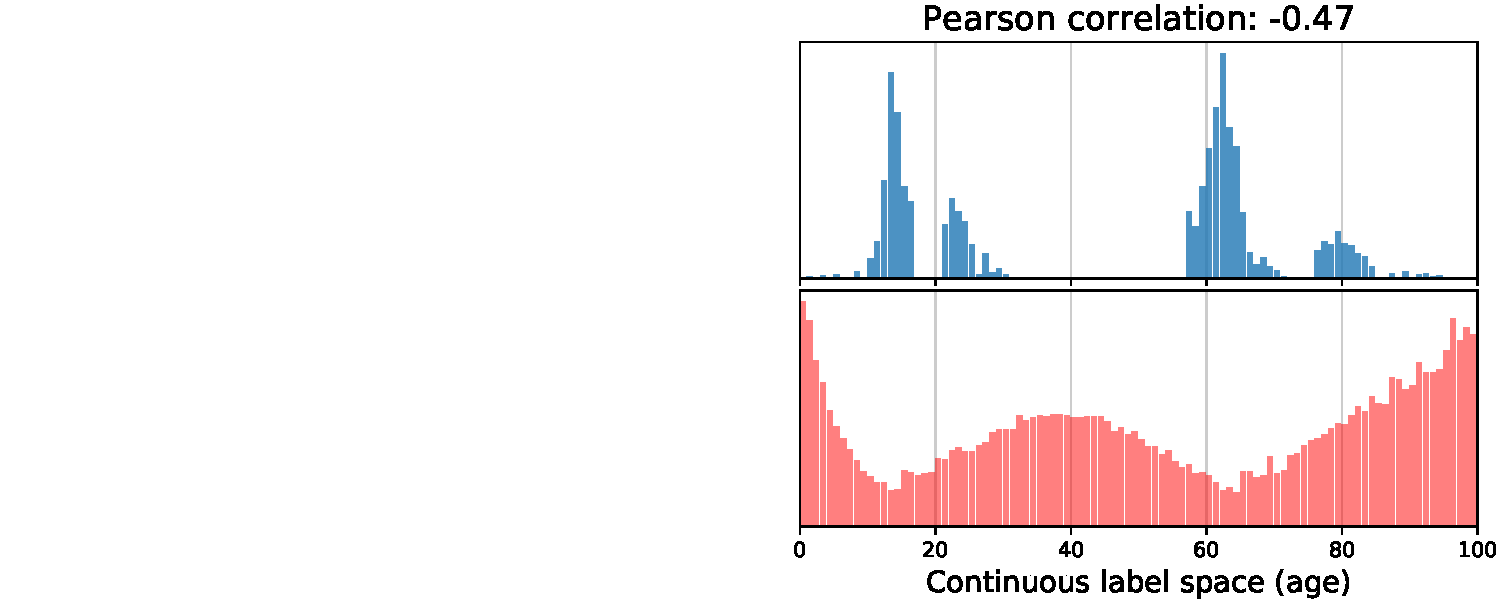
\includegraphics[width=\linewidth]{images/err_motivate_1_right.pdf}
		\caption{IMDB-WIKI (subsampled)}
	\end{subfigure}
	%\caption{}
	\end{figure}
	\credit{Image}{yang2021delving}
\end{frame}

%\section{References}
%\begin{frame}[allowframebreaks]
%\frametitle{References}
%\printbibliography
%\end{frame}

\end{document}